%% %%%%%%%%%%%%%%%%%%%%%%%%%%%%%%%%%%%%%%%%%%%%%%%%%
%% Template for a conference paper, prepared for the
%% Food and Resource Economics Department - IFAS
%% UNIVERSITY OF FLORIDA
%% %%%%%%%%%%%%%%%%%%%%%%%%%%%%%%%%%%%%%%%%%%%%%%%%%
%% Version 1.0 // November 2019
%% %%%%%%%%%%%%%%%%%%%%%%%%%%%%%%%%%%%%%%%%%%%%%%%%%
%% Ariel Soto-Caro
%%  - asotocaro@ufl.edu
%%  - arielsotocaro@gmail.com
%% %%%%%%%%%%%%%%%%%%%%%%%%%%%%%%%%%%%%%%%%%%%%%%%%%
\documentclass[11pt]{article}
\usepackage{UF_FRED_paper_style}
\usepackage{xcolor}  % colored text
\usepackage{lipsum}  %% Package to create dummy text (comment or erase before start)
\usepackage{booktabs}  % professional-quality tables
\usepackage{caption}
\usepackage{subcaption}
%\usepackage{emoji}
\usepackage{float}
\usepackage{geometry}


%% ===============================================
%% Setting the line spacing (3 options: only pick one)
% \doublespacing
% \singlespacing
\onehalfspacing
%% ===============================================

\setlength{\droptitle}{-5em} %% Don't touch

% %%%%%%%%%%%%%%%%%%%%%%%%%%%%%%%%%%%%%%%%%%%%%%%%%%%%%%%%%%
% SET THE TITLE
% %%%%%%%%%%%%%%%%%%%%%%%%%%%%%%%%%%%%%%%%%%%%%%%%%%%%%%%%%%

% TITLE:
\title{Sentiment Analysis Domain Transfer}

% AUTHORS:
\author{Kevin Willer\\% Name author
    \href{mailto:kwiller@uni-potsdam.de}{\texttt{kwiller@uni-potsdam.de}} %% Email author 1 
    }
    
% DATE:
\date{\today}

% %%%%%%%%%%%%%%%%%%%%%%%%%%%%%%%%%%%%%%%%%%%%%%%%%%%%%%%%%%
% %%%%%%%%%%%%%%%%%%%%%%%%%%%%%%%%%%%%%%%%%%%%%%%%%%%%%%%%%%
\begin{document}
% %%%%%%%%%%%%%%%%%%%%%%%%%%%%%%%%%%%%%%%%%%%%%%%%%%%%%%%%%%
% %%%%%%%%%%%%%%%%%%%%%%%%%%%%%%%%%%%%%%%%%%%%%%%%%%%%%%%%%%
% ABSTRACT
% %%%%%%%%%%%%%%%%%%%%%%%%%%%%%%%%%%%%%%%%%%%%%%%%%%%%%%%%%%
% %%%%%%%%%%%%%%%%%%%%%%%%%%%%%%%%%%%%%%%%%%%%%%%%%%%%%%%%%%
{\setstretch{.8}
\maketitle
% %%%%%%%%%%%%%%%%%%
\begin{abstract}
% CONTENT OF ABS HERE--------------------------------------

  abstract goes here abstract goes here abstract goes here abstract goes here abstract goes here abstract goes here abstract goes here abstract goes here abstract goes here abstract goes here abstract goes here abstract goes here abstract goes here abstract goes here abstract goes here abstract goes here abstract goes here abstract goes here abstract goes here abstract goes here abstract goes here abstract goes here abstract goes here abstract goes here

% END CONTENT ABS------------------------------------------
\noindent
\textit{\textbf{Keywords: }%
Sentiment Analysis; Twitter; Transformer; Domain Transfer; Stance Detection} \\ %% <-- Keywords HERE!
\noindent

\end{abstract}
}
\clearpage
\tableofcontents
\clearpage
% %%%%%%%%%%%%%%%%%%%%%%%%%%%%%%%%%%%%%%%%%%%%%%%%%%%%%%%%%%
% %%%%%%%%%%%%%%%%%%%%%%%%%%%%%%%%%%%%%%%%%%%%%%%%%%%%%%%%%%
% BODY OF THE DOCUMENT
% %%%%%%%%%%%%%%%%%%%%%%%%%%%%%%%%%%%%%%%%%%%%%%%%%%%%%%%%%%
% %%%%%%%%%%%%%%%%%%%%%%%%%%%%%%%%%%%%%%%%%%%%%%%%%%%%%%%%%%
\section{Introduction \& Related Work}
In 2008 a technical Whitepaper was pseudonymously released (\citet{bitcoin}). Taking elements from peer-to-peer and cryptographic technology and combining them into the idea of a distributed ledger called the Blockchain, it described the first truly decentralized currency: Bitcoin. Since then, global interest in the capabilities and possibilities for Blockchain technologies has grown immensely. Meanwhile the underlying technology has also evolved a lot and, by now, is used for many more things than the creation of mere currencies. Despite this, the nature of the need for a type of "Currency" in the context of the Blockchain validation mechanics, has brought forth an ever-growing number of Cryptocurrencies and tokens, which are freely traded in centralized and decentralized exchanges and due to their relative lack of regulation and immense volatility, have attracted investors, traders and speculators on a global scale. \\

\section{table test}

\begin{table}[H]
\renewcommand{\arraystretch}{1.2}
\centering
\caption{\label{table:example-tweets} Some examples of idiosyncratic language used on Crypto-Twitter.}
\begin{tabular}{lll}
\textbf{Tweet Excerpts} & \textbf{Rough Paraphase} & \textbf{Sentiment}  \\ \midrule
"Pump to the moon " & Strong price appreciation. & Positive   \\
"Don't chase FOMO pumps  & Buying high leads to loss. & Negative\\
or you will get rekt" & & \\
"No more FUD" & No spreading of neg. sentiment. & Positive\\
"LFGGGGG " & Extreme price appreciation. & Positive \\
"Just aped in." & Invested based on emotion. & Neutr./Positive \\
"RELAX HODL \#BabyDoge" & Longer term investment. & Positive \\
\bottomrule
\end{tabular}
\end{table}

\section{fig test}

\begin{figure}[H]
\centering
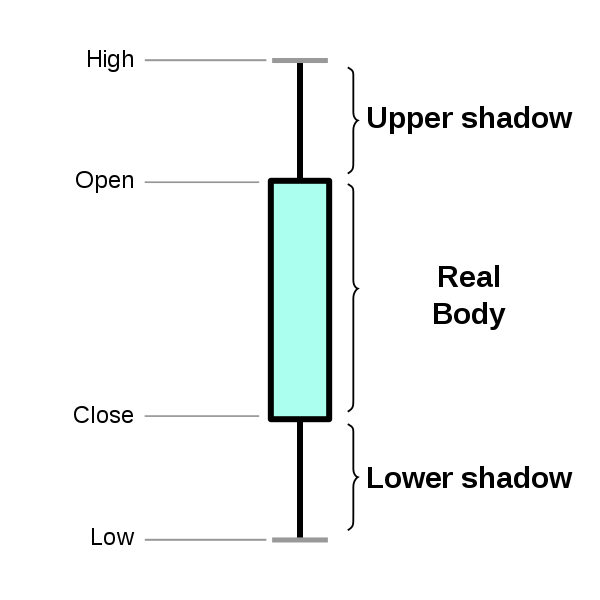
\includegraphics[scale=0.2]{figures/candlestickwiki.png}
\caption {Kline Candlestick. (Source: en.wikipedia.org/wiki/Candlestick\_chart)}
\label{fig:candlestick}
\end{figure}

% %%%%%%%%%%%%%%%%%%%%%%%%%%%%%%%%%%%%%%%%%%%%%%%%%%%%%%%%%%
% %%%%%%%%%%%%%%%%%%%%%%%%%%%%%%%%%%%%%%%%%%%%%%%%%%%%%%%%%%
% REFERENCES SECTION
% %%%%%%%%%%%%%%%%%%%%%%%%%%%%%%%%%%%%%%%%%%%%%%%%%%%%%%%%%%
% %%%%%%%%%%%%%%%%%%%%%%%%%%%%%%%%%%%%%%%%%%%%%%%%%%%%%%%%%%
\medskip

\bibliography{references.bib} 


% ==========================
% ==========================
% ==========================


\end{document}
